\documentclass[12pt]{report}

\usepackage{amssymb, fullpage, amsmath}
\usepackage{graphicx}

\newtheorem{problem}{Problem}

\newenvironment{solution}[1][\it{Solution}]{\textbf{#1. } }{$\square$}

\graphicspath{ {./} }

\pagestyle{empty}

\def\Z{{\mathbb Z}}
\def\Q{{\mathbb Q}}
\def\C{{\mathbb C}}
\def\R{{\mathbb R}}
\def\N{{\mathbb N}}

\begin{document}

\large

\begin{center}
 Math 584 Homework 2\\
 Due Next Wednesday\\
 By Marvyn Bailly\\
\end{center}

\normalsize

\hrule

%---------------%
%---Problem 1---%
%---------------%

%--status--$

\begin{problem}
    Exercise 3.2
\end{problem}

\begin{solution}
    \noindent
    Let $A \in \C^{m\times m}$ and let $x \neq \vec{0}$ be the eigenvector corresponding to the largest eigenvalue of $A$, $\lambda$. Let 
    $\rho (A)$ is the spectral radius of $A$. Notice that by letting $||\cdot||$ be any norm of $\C^m$ we get,
    \begin{align*}
        \lambda x &= Ax\\
        ||\lambda x|| &= ||Ax||\\
        |\lambda| ||x|| &= ||Ax||\\
        |\lambda| &= \frac{||Ax||}{||x||}\\
        |\lambda| &\leq \sup_{||x|| = 1} \frac{||Ax||}{||x||} = ||A||\\
    \end{align*}
    Therefore $\rho(A) \leq ||A||$.
\end{solution}

%----------------------------------------------------------------------------------------------------%
%\vskip 20pt
%\newpage

%---------------%
%---Problem x---%
%---------------%

%--status--$

\begin{problem}
    Exercise 3.3
\end{problem}

\begin{solution}
    \noindent
    Let $x \in \C^m$ and $A \in \C^{m \times n}$
    \begin{enumerate}
        \item [a.] We can show that $\|x\|_\infty \leq \|x\|_2$ by considering that, $\|x\|_\infty = \max_{1 \leq i \leq m} |x_i|  \implies (\|x\|_\infty)^2 = \max_{1 \leq i \leq m}|x_i^2|$ but $(\|x\|_\infty)^2 \leq \sum_{j=1}^m(x_j^2)$ so $\|x\|_\infty \leq \left( \sum_{j=1}^m(x_j^2) \right)^\frac{1}{2} = \| x \|_2$. An example of equality is when $x = e_1$. Then $\|x\|_\infty = 1 = \|x\|_2$. 
        \item [b.] We can show that $\|x\|_2 \leq \sqrt{m}\|x\|_\infty$ when considering that $\| x \|_2 = \left( \sum_{j=1}^m |x_j|\right)^\frac{1}{2} = \left( |x_1|^2 + |x_2|^2 + \cdots + |x_m|^2 \right)^\frac{1}{2} \leq \left( \max_{1 \leq i \leq m} |x_i|^2 + \max_{1 \leq i \leq m} |x_i|^2 + \cdots + \max_{1 \leq i \leq m} |x_i|^2\right)^\frac{1}{2} = \sqrt{m}\|x\|_\infty$. An example of equality is when $x = ( 1,1 )^T$ then $\|x\|_2 = \sqrt{2} = \sqrt{2} (1) = \|x\|_\infty$.
        \item [c.] We can show that $\|A\|_\infty \leq \sqrt{n} \|A\|_2$ by recalling that $\|A\|_\infty = \max_{1 \leq j \leq m}\|a_i\|_1$. From (a) we have that $|Ax|_\infty \leq \|Ax\|_2$ and from (b) we have that $\frac{1}{\sqrt{n}}\|x\|_2 \leq \|x\|_\infty$. Combining these facts we get $$\frac{\|Ax\|_\infty}{\|x\|_\infty} \leq \frac{\|Ax\|_2}{\frac{1}{n}\|x\|_2}$$ taking the supremum of both sides we get $\|A\|_\infty \leq \sqrt{n} \|A\|_2$. An example of equality is given when $A = \begin{pmatrix} 1&1\\0&0 \end{pmatrix}$. Then the max row sum is $2$ and the two norm of $A$ is $\sqrt{2}$, thus we have that $\|A\|_\infty = 2 = \sqrt{2} \|A\|_2 = \sqrt{2}\sqrt{2} = 2$.
        \item [d.] To show that $\|A\|_2 \leq \sqrt{m} \| A \|_\infty$ recall that (a) states that $\|x\|_\infty \leq \|x\|_2$ and (b) gives that $\|Ax\|_2 \leq \sqrt{m} \|Ax\|_\infty$. Using these two facts we have that $$\frac{\|Ax\|_2}{\|x\|_2} \leq \frac{\sqrt{m}\|Ax\|_\infty}{\|x\|_\infty}.$$ Taking the supremum of both sides we get $\|A\|_2 \leq \sqrt{m} \| A \|_\infty$. An example of equality is given by the $2\times 2$ identity matrix, $I_2$. Since $I_2$ is diagonal, we know that $\|I_2\|_2 = \sqrt{1 + 1}  = \sqrt{2}$. And the max row sum of $I_2$ is $1$, thus we have $\sqrt{2} = 1 \sqrt{2}$. $\|A\|_2 = \sqrt{2} = \sqrt{2} \| A \|_\infty = \sqrt{2}$
    \end{enumerate}
\end{solution}

%----------------------------------------------------------------------------------------------------%
%\vskip 20pt
%\newpage

%---------------%
%---Problem x---%
%---------------%

%--status--$

\begin{problem}
    Exercise 4.1
\end{problem}

\begin{solution}
    \noindent
    We wish to compute the following SVDs
    \begin{enumerate}
        \item [a] Consider the matrix $$A = \begin{pmatrix} 3&0\\0&-2\end{pmatrix}.$$ Consider $Ax$, then $A$ stretches values along $x_1$ by three and flips $x_2$ before stretching it by $2$. Thus $A$ begins by not rotating, $\begin{pmatrix} 1&0\\0&1\end{pmatrix}$, then stretches, $\begin{pmatrix} 3&0\\0&2\end{pmatrix}$, and finally rotates to flip $x_2$,$\begin{pmatrix} 1&0\\0&-1\end{pmatrix}$. Therefore we can geometrically construct an SVD to be, $$A = \begin{pmatrix} 1&0\\0&-1\end{pmatrix}\begin{pmatrix} 3&0\\0&2\end{pmatrix}\begin{pmatrix} 1&0\\0&1\end{pmatrix}$$
        
        \item [b] Consider the matrix $$A = \begin{pmatrix} 2&0\\0&3 \end{pmatrix}.$$ Consider $Ax$, then $A$ stretches values along $x_1$ by $2$ and $x_2$ by $3$ without rotating. Thus we have that the singular values are $3,2$. Note that we have to flip the corresponding eigenvectors to match the ordering of the singular values. Therefore we can geometrically construct an SVD to be, $$A = \begin{pmatrix} 0&1\\1&0\end{pmatrix}\begin{pmatrix} 3&0\\0&2\end{pmatrix}\begin{pmatrix} 0&1\\1&0\end{pmatrix}$$
        
        \item [c] Consider the matrix $$A = \begin{pmatrix} 0&2\\0&0\\0&0 \end{pmatrix}.$$ Then $Ax$ maps $x_1$ to two times $x_2$ while $x_2$ is mapped to $0$. Thus the singular values are $2,0$. So $A$ begins by rotating so that $x_2$ goes to $x_1$, stretches by the singular values, and then does not rotate. Therefore we can geometrically construct an SVD to be, $$A = \begin{pmatrix} 1&0\\0&1\\0&0\end{pmatrix}\begin{pmatrix} 2&0\\0&0\end{pmatrix}\begin{pmatrix} 0&1\\1&0\end{pmatrix}.$$ 
        
        \item [d] Consider the matrix $$A = \begin{pmatrix} 1&1\\0&0 \end{pmatrix}.$$ Here $Ax$ is mapping $x_1$ to $x_1 + x_2$ while $x_2$ goes to zero. This means that we begin by rotating $\pi/4$, then magnifying by $\sqrt{2}$, and then not rotating anymore. Putting these ideas together, we can construct the SVD geometrically to be,
        $$A = \begin{pmatrix} 1&0\\0&1\end{pmatrix}\begin{pmatrix} \sqrt{2}&0\\0&0\end{pmatrix}\begin{pmatrix} \frac{\sqrt{2}}{2}&\frac{\sqrt{2}}{2}\\-\frac{\sqrt{2}}{2}&\frac{\sqrt{2}}{2}\end{pmatrix}.$$ 
        
        \item [e] Consider the matrix $$A = \begin{pmatrix} 1&1\\1&1 \end{pmatrix}.$$ Then $Ax$ scales $x_1$ and $x_2$ to $x_1 + x_2$. So we begin by rotating 45 degrees, magnifying by $2$, and then finally rotating again to match the basis. Thus we can geometrically construct the SVD to be, $$A = \begin{pmatrix} \frac{\sqrt{2}}{2}&-\frac{\sqrt{2}}{2}\\\frac{\sqrt{2}}{2}&\frac{\sqrt{2}}{2}\end{pmatrix}\begin{pmatrix} 2&0\\0&0\end{pmatrix}\begin{pmatrix} \frac{\sqrt{2}}{2}&\frac{\sqrt{2}}{2}\\-\frac{\sqrt{2}}{2}&\frac{\sqrt{2}}{2}\end{pmatrix}.$$
    \end{enumerate}
\end{solution}

%----------------------------------------------------------------------------------------------------%
%\vskip 20pt
%\newpage

%---------------%
%---Problem x---%
%---------------%

%--status--$

\begin{problem}
    Exercise 4.5
\end{problem}

\begin{solution}
    \noindent
    Let $A \in \C^{m\times n}$. By theorem 4.1, we know that there exists  singular value decomposition of $A = U\Sigma V^*$ where $U \in \C^{m\times m}$ is unitary, $V \in \C^{n\times n}$ is unitary, and $\Sigma \in \R^{m\times m}$. We wish to show that if $A \in \R^{m\times n}$ then so is $U$ and $V$. Notice that
    $$A^*A = (U\Sigma V^*)^*U\Sigma V^* = V\Sigma U U^* \Sigma V^* = V \Sigma V^*.$$
    Since $AA^*$ is Hermitian, we know that it has real eigenvalues from the previous homework. If we let $\lambda_i \in \R$ be the $i$th eigen value with $v_i$ be the corresponding eigenvector, then
    \begin{align*}
        &A^*Av_i = \lambda_i v_i\\
        \implies &(A^*A - \lambda_i)v_i = 0  
    \end{align*} 
    Since $(A^*A - \lambda i)$ is real, $v_i$ must also be real in order to preserve the product being zero. Thus the eigenvectors of $AA^*$ are real. From theorem 4.1, this implies that the values of $V$ must be real and therefore $V^*$ is also real. When considering $A^*A$, we can construct a similar argument to show that $U$ is made from the real eigenvectors of $A^*A$. Therefore, $U$ and $V$ are both real matrices and we have shown that the SVD of $A$ is real.  
\end{solution}

%----------------------------------------------------------------------------------------------------%
%\vskip 20pt
%\newpage


%---------------%
%---Problem x---%
%---------------%

%--status--$

\begin{problem}
    Exercise 5.4
\end{problem}

\begin{solution}
    \noindent
    Let $A \in \C^{m \times m}$ and let its SVD be $A = U \Sigma V^*$. Note that $U,V$ have linearly independent columns and are unitary. Consider the matrix $$\begin{pmatrix} 0 & A^* \\ A & 0 \end{pmatrix}$$
    which is a $2m \times 2m$ Hermitian matrix. Consider that $AV = V\Sigma$ and $A^*U=V\Sigma$. This gives us,
    $$\begin{pmatrix}
        0&A^*\\A&0\\
    \end{pmatrix}\begin{pmatrix}
        V\\U
    \end{pmatrix}=\begin{pmatrix}
        V\Sigma\\U\Sigma
    \end{pmatrix}$$
    and 
    $$\begin{pmatrix}
        0&A^*\\A&0\\
    \end{pmatrix}\begin{pmatrix}
        -V\\U
    \end{pmatrix}=\begin{pmatrix}
        V\Sigma\\-U\Sigma
    \end{pmatrix}$$
    Putting these together we get,
    $$\begin{pmatrix}
        0&A^*\\A&0\\
    \end{pmatrix}\begin{pmatrix}
        V&V\\U&-U
    \end{pmatrix}=\begin{pmatrix}
        V\Sigma&&V\Sigma\\U\Sigma&&-U\Sigma
    \end{pmatrix}=\begin{pmatrix}
        V&V\\U&-U\\
    \end{pmatrix}\begin{pmatrix}
        \Sigma&0\\0&\Sigma
    \end{pmatrix}$$
    Which implies that
    $$\begin{pmatrix}
        0&A^*\\A&0\\
    \end{pmatrix}\begin{pmatrix}
        V&-V\\U&U
    \end{pmatrix} = \begin{pmatrix}
        V&-V\\U&U\\
    \end{pmatrix}\begin{pmatrix}
        \Sigma&0\\0&-\Sigma
    \end{pmatrix}$$
    And since $V$ and $U$ are unitary,
    $$\begin{pmatrix}
        0&A^*\\A&0\\
    \end{pmatrix} = \begin{pmatrix}
        V&-V\\U&U\\
    \end{pmatrix}\begin{pmatrix}
        \Sigma&0\\0&-\Sigma
    \end{pmatrix}
    \begin{pmatrix}
        V&-V\\U&U
    \end{pmatrix}^{-1} = X \Lambda X^{-1}$$
    Where $\Sigma$ and $-\Sigma$ are diagonal matrices with eigenvalues as entries. 
\end{solution}

%----------------------------------------------------------------------------------------------------%
%\vskip 20pt
%\newpage

\begin{problem}
    Matlab Fun
\end{problem}

\begin{solution}
    \begin{figure}
        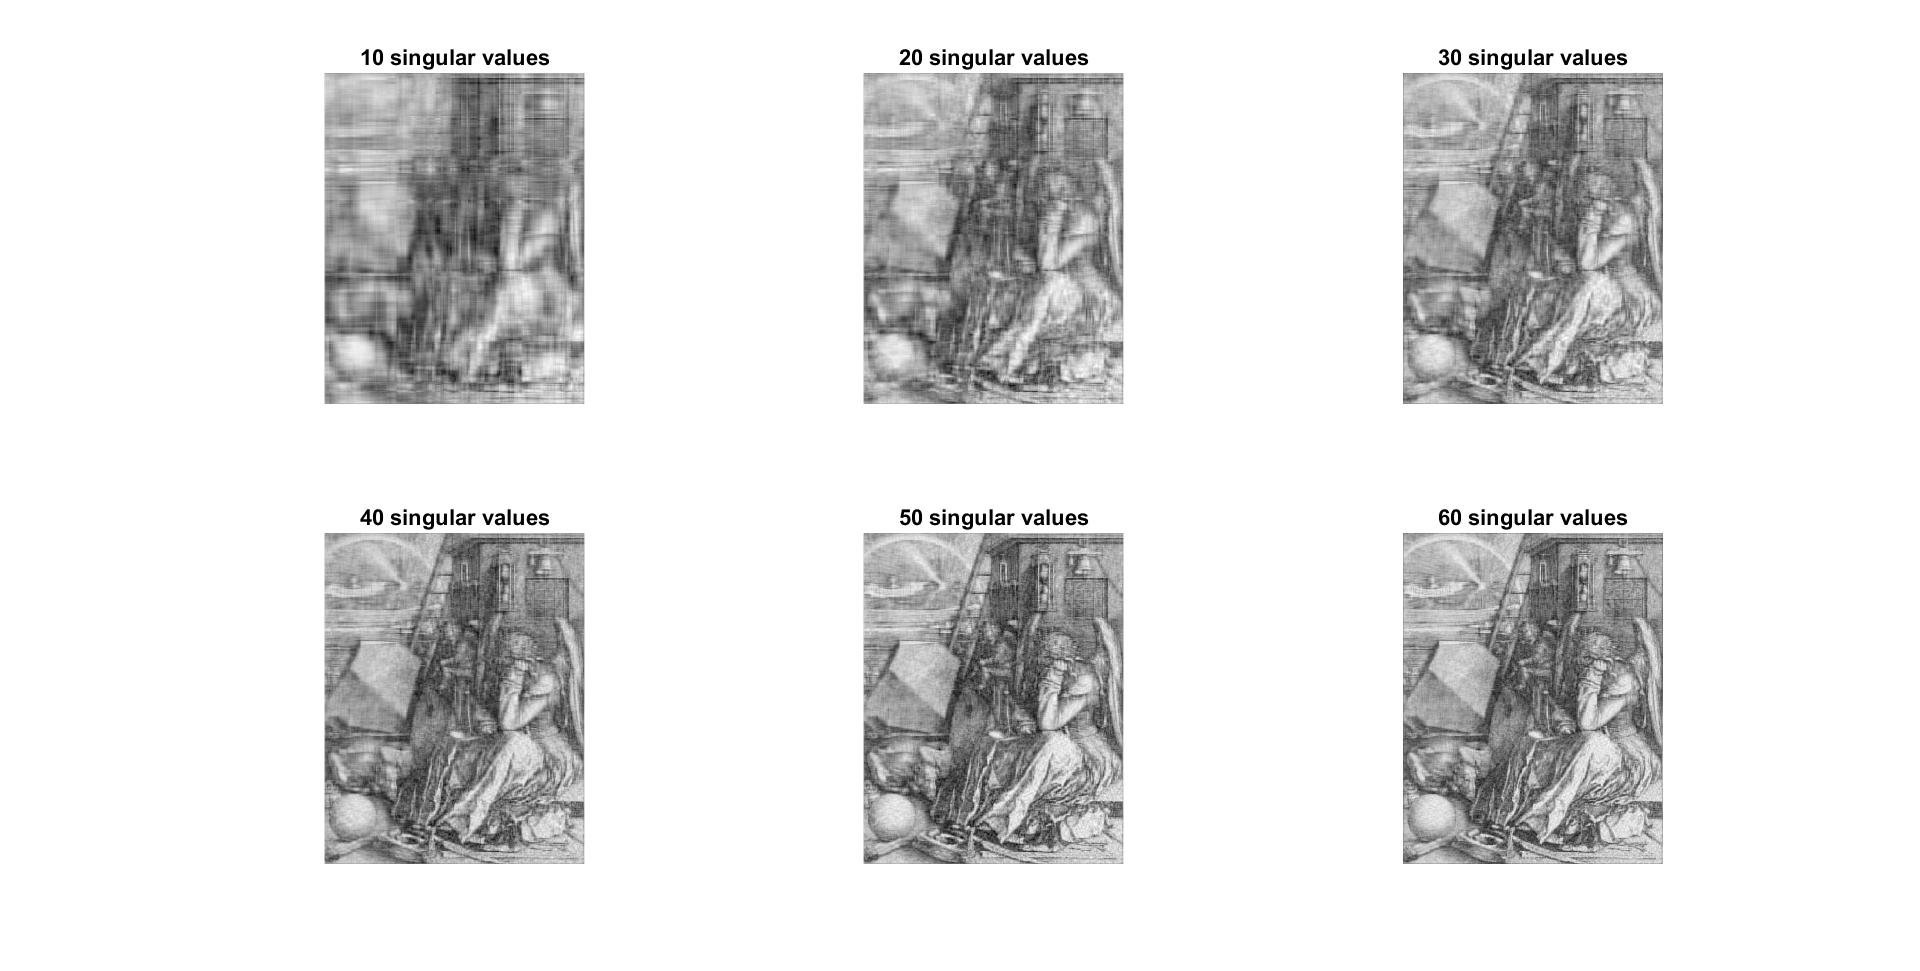
\includegraphics[width=\linewidth]{hw2.jpg}
        \caption{A boat.}
        \label{fig:boat1}
      \end{figure}
\end{solution}

\end{document}